\documentclass[12pt]{article}

\usepackage{fullpage}
\usepackage{multicol,multirow}
\usepackage{tabularx}
\usepackage{ulem}
\usepackage[utf8]{inputenc}
\usepackage[russian]{babel}
\usepackage{amsmath}
\usepackage{amssymb}

\usepackage{graphicx}
\DeclareGraphicsExtensions{.png}

\usepackage{titlesec}

\titleformat{\section}
  {\normalfont\Large\bfseries}{\thesection.}{0.3em}{}

\titleformat{\subsection}
  {\normalfont\large\bfseries}{\thesubsection.}{0.3em}{}

\titlespacing{\section}{0pt}{*2}{*2}
\titlespacing{\subsection}{0pt}{*1}{*1}
\titlespacing{\subsubsection}{0pt}{*0}{*0}
\usepackage{listings}
\lstloadlanguages{Lisp}
\lstset{extendedchars=false,
	breaklines=true,
	breakatwhitespace=true,
	keepspaces = true,
	tabsize=2
}
\begin{document}


\section*{Отчет по лабораторной работе №\,3 
по курсу \guillemotleft  Функциональное программирование\guillemotright}
\begin{flushright}
Студент группы 8О-307 МАИ \textit{Вельтман Лина}, \textnumero 7 по списку \\
\makebox[7cm]{Контакты: {\tt  kluuo@mail.ru} \hfill} \\
\makebox[7cm]{Работа выполнена: 5.04.2020 \hfill} \\
\ \\
Преподаватель: Иванов Дмитрий Анатольевич, доц. каф. 806 \\
\makebox[7cm]{Отчет сдан: \hfill} \\
\makebox[7cm]{Итоговая оценка: \hfill} \\
\makebox[7cm]{Подпись преподавателя: \hfill} \\

\end{flushright}

\section{Тема работы}
Последовательности, массивы и управляющие конструкции Коммон Лисп.

\section{Цель работы}
Научиться создавать векторы и массивы для представления матриц, освоить общие функции работы с последовательностями, инструкции цикла и нелокального выхода.

\section{Задание (вариант №46)}
Запрограммировать на языке Коммон Лисп функцию, принимающую в качестве единственного аргумента целое число {\tt n} - порядок матрицы. Функция должна создавать и возвращать двумерный массив представляющий целочисленную квадратную матрицу порядка n, элементами которой являются числа {\tt $1, 2, ..., n^{2}$}, расположенные по спирали.\\

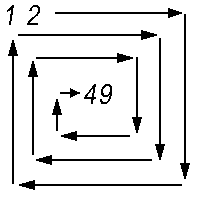
\includegraphics {spiralmatrix.png}\\

\section{Оборудование ПЭВМ студента}
Ноутбук MacBook Pro (13-inch, 2017), процессор 2.3GHz Intel Core i5, память: 8Gb, разрядность системы: 64.

\section{Программное обеспечение ЭВМ студента}
macOS Catalina 10.15.4, реализация языка SBCL 1.4.16, текстовый редактор Sublime Text 3.

\section{Идея, метод, алгоритм}

Заполнение матрицы происходит по столбцам, а затем по строкам поочередно. Сначала проходим по столбцам слева-направо (причем при каждом заполнении увеличиваем счетчик на единицу, что позволяет выполнить условие, при котором элементами матрицы являются числа от единицы до квадрата исходного числа n), пока не достигнем границы матрицы. Дойдя до пограничного элемента, мы спускаемся на один элемент и проходим уже по строкам сверху-вниз, заполняя каждый элемент матрицы. Опять достигнув пограничного элемента матрицы, мы начинаем двигаться снова по столбцам, но уже меняем направление: справа-налево. Дойдя до границы, начинаем двигаться по строкам, но уже сверху-вниз. Далее алгоритм повторяется сначала. Стоит отметить, что проверяются не только границы матрицы, но и был ли уже заполнен выбранный элемент, если одно из этих условий выполняется, то переменным, отвечающим за шаги по столбцам и строкам присваиваются новые значения (а именно: шагу по столбцам присваивается значение шага по строкам с минусом, а шагу по строкам присваивается еще неизмененное значение шага по столбцам), а не просто инкрементируются.

\section{Сценарий выполнения работы}

\section{Распечатка программы и её результаты}

\subsection{Исходный код}
\lstinputlisting{lab3_46.lisp}

\subsection{Результаты работы}
\lstinputlisting{log.txt}

\section{Дневник отладки}
\begin{tabular}{|c|c|c|c|}
\hline
Дата & Событие & Действие по исправлению & Примечание \\
\hline
\end{tabular}

\section{Замечания автора по существу работы}
Было интересно вспомнить работу с двумерными матрицами и их обходом, выявлять закономерности, которые помогут упростить алгоритм.

\section{Выводы}
Во время выполнения данной лабораторной я познакомилась с массивами в языке {\tt Common Lisp}, а также узнала, как выполнять различные операции над ними, как использовать циклы. Массивы являются основополагающей структурой данных в программировании и часто используются, потому что в них удобно хранить данные, поэтому важно уметь работать с ними в любом языке программирования.

\end{document}